

\chapter{가설 검정 (Hypothesis testing)}
\label{testing}

이번 장에서 사용되는 코드는 {\tt hypothesis.py}에 있다.
코드를 다운로드하고 작업하는 것에 대한 정보는 ~\ref{code}을 참조한다.


\section{전통적 가설 검정 (Classical hypothesis testing)}
\index{가설 검정 (hypothesis testing)}
\index{외관 효과 (apparent effect)}

NSFG에서 데이터를 탐색하면서, 첫째 아이와 첫째가 아닌 아이들 간 차이를 
포함해서 몇가지 ``외관 효과 (apparent effects)''를 봤다.
지금까지 액면 그대로 이러한 효과를 받아들였다; 이번 장에서 이를 검정한다. 

\index{국가 가정 성장 조사 (National Survey of Family Growth)}
\index{NSFG}

다루고자 하는 근본적인 질문은 표본에서 본 효과가 더 큰 모집단에서 나타날 것인가다.
예를 들어, NSFG 표본에서 첫째 아이와 첫째 아이가 아닌 아이들에 대한 평균 임신 기간에
차이를 봤다. 알고자 하는 것은 이 효과가 미국 여성에 대한 진정한 차이를 반영하는지 
혹은, 우연히 표본에서 생겨난 것이냐다.
\index{임신 기간 (pregnancy length)} 
\index{기간 (length)!임신 (pregnancy)}

피셔 귀무 가설 검정(Fisher null hypothesis testing), 네이만 피어슨 의사결정 이론(Neyman-Pearson decision theory), 베이즈 추론(Bayesian inference)\footnote{베이즈 추론에 대한 좀더 많은 정보는 후속해서 출간되는 {\it Think Bayes}를 참조한다.}을 포함해서 질문을 구성하는 방법이 몇가지 있다.
여기 제시하는 것은 대부분의 사람이 실무에서 사용하는 세가지 방법의 일부분으로 {\bf 전통적 가설 검정 (classical hypothesis testing)}이라고 저자가 작명한 것이다.
\index{베이즈 추론 (Bayesian inference)}
\index{귀무 가설 (null hypothesis)}

전통적 가설 검정의 목적은 다음 질문에 답하는 것이다.
``표본과 명백한 효과가 주어졌다면, 우연히 그런 효과를 목도하는 확률이 얼마인가?''
다음에 질문에 답을 하는 방법이 있다.

\begin{itemize}

\item 첫번째 단계는 {\bf 검정 통계량 (test statistic)}을 선택해서 
외관 효과 크기를 정량화한다. NSFG 예제에서, 명백한 효과는 첫번째 아이와 첫째가 아닌 아이들 사이에 임신 기간에 차이가 된다. 그래서, 검정 통계량에 대한 자연스러운 선택이
두 집단 사이에 평균 차이가 된다.
  \index{검정 통계량 (test statistic)}

\item 두번째 단계는 {\bf 귀무 가설 (null hypothesis)}을 정의하는 것으로,
명백한 효과가 사실이 아니라는 가정에 기반한 시스템 모형이다.
NSFG 예제에서, 귀무 가설은 첫째 아이와 첫째가 아닌 아이들 사이에 차이가 없다가 된다;
즉, 두 집단 임신 기간은 동일한 분포다. 
\index{귀무 가설 (null hypothesis)}
\index{임신 기간 (pregnancy length)}
\index{모형 (model)}

\item 세번째 단계는 {\bf p-값(p-value)}을 계산하는 것으로, 만약 귀무 가설이 사실이라면 명백한 효과를 볼 확률값이 된다. NSFG 예제에서, 평균에 실제 차이를 계산하고 나서, 귀무 가설 아래에서 차이를 크게 혹은 더 크게 볼 확률을 계산한다.
\index{p-값 (p-value)}

\item 마지막 단계는 결과를 해석하는 것이다. 만약 p-값이 낮다면, 효과에 
{\bf 통계적 유의성 (statistically significant)}이 있다고 한다.
우연히 발생할 것 같지 않다는 의미가 된다. 이 경우 더 큰 모집단에서 효과가 나타날 것 같다고 추론한다.\index{통계적 유의성 (statistically significant)} 
\index{유의성 (significant)}

\end{itemize}

이 과정의 로직(logic)은 모순(contradiction)에 의한 증명과 유사하다. 
수학 명제(mathematical statement) A를 증명하기 위해, 일시적으로 A 가 거짓이라고 가정한다.
만약 가정이 모순을 이끌게 되면, A 는 사실 참이어야 한다고 결론낸다.

\index{모순, 증명 (contradiction, proof by)}
\index{모순에 의한 증명 (proof by contradiction)}

유사하게, ``효과가 사실 (This effect is real)'' 같은 가설을 검정하기 위해서,
일시적으로 효과가 없다고 가정한다. 이것이 귀무가설이다.
이 가정에 기반해서, 외관 효과 확률을 계산한다. 이것이 p-값이다.
만약 p-값이 작다면, 귀무 가설이 사실이 아닐 것 같다고 결론낸다.

\index{p-값 (p-value)}
\index{귀무 가설 (null hypothesis)}


\section{HypothesisTest}
\label{hypotest}
\index{평균 (mean)!차이 (difference in)}

{\tt thinkstats2}에는 전통적 가설 검정 구조를 표현하는 {\tt HypothesisTest} 클래스가 있다.

다음에 클래스 정의가 있다.
\index{HypothesisTest}

\begin{verbatim}
class HypothesisTest(object):

    def __init__(self, data):
        self.data = data
        self.MakeModel()
        self.actual = self.TestStatistic(data)

    def PValue(self, iters=1000):
        self.test_stats = [self.TestStatistic(self.RunModel()) 
                           for _ in range(iters)]

        count = sum(1 for x in self.test_stats if x >= self.actual)
        return count / iters

    def TestStatistic(self, data):
        raise UnimplementedMethodException()

    def MakeModel(self):
        pass

    def RunModel(self):
        raise UnimplementedMethodException()
\end{verbatim}

{\tt HypothesisTest}는 추상 부모 클래스로 메쏘드 몇개에 대한 완전한 정의와 
다른 메쏘드를 위한 자리잡기(place-keeper) 기능 제공한다.
{\tt HypothesisTest}에 기반한 자식 클래스는 \verb"__init__"와 {\tt PValue} 을 상속받고, {\tt TestStatistic}, {\tt RunModel}, 그리고 선택옵션으로 {\tt MakeModel} 메쏘드를 제공한다.
\index{HypothesisTest}

\verb"__init__"은 적절한 어떤 형식의 데이터도 받아들인다.
{\tt MakeModel} 호출해서 귀무 가설을 표현을 구축하고 나서,
데이터를 {\tt TestStatistic}에 전달하고 표본 효과 크기를 계산한다.

\index{검정 통계량 (test statistic)}
\index{귀무 가설 (null hypothesis)}

{\tt PValue}는 귀무 가설 아래에서 외관 효과 확률을 계산한다.
매개 변수로 {\tt iters}을 받는데 실행할 모의 시험 횟수다.
첫번째 행은 모의 시험 데이터를 생성하고, 검정 통계량을 계산하고, 
\verb"test_stats"에 저장한다.
결과는 관측된 검정 통계량 {\tt self.actual}와 동일하거나 큰 \verb"test_stats" 에 있는 비율이다.
\index{모의 시험 (simulation)}

간단한 예제\footnote{인용 출처: MacKay, {\it Information
Theory, Inference, and Learning Algorithms}, 2003.}로, 250번 동전을 던져서 앞면 140회, 뒷면 110회 나왔다고 가정하자.
이 결과에 기초하여, 동전에 편의가 있는지 의심할지도 모른다; 즉, 좀더 앞면이 나올 것 같다.
이 가설을 검정하기 위해서, 확률을 계산해서 만약 동전이 정말 공정하다면, 그런 차이가 있는지 살펴본다.

\index{편의 동전 (biased coin)}
\index{MacKay, David}

\begin{verbatim}
class CoinTest(thinkstats2.HypothesisTest):

    def TestStatistic(self, data):
        heads, tails = data
        test_stat = abs(heads - tails)
        return test_stat

    def RunModel(self):
        heads, tails = self.data
        n = heads + tails
        sample = [random.choice('HT') for _ in range(n)]
        hist = thinkstats2.Hist(sample)
        data = hist['H'], hist['T']
        return data
\end{verbatim}

모수 {\tt data}는 정수 짝이다: 앞면 숫자, 뒷면 숫자.
검정 통계량은 둘 사이 절대값 차이다. 그래서 {\tt self.actual}은 30 이다.
\index{HypothesisTest}

{\tt RunModel}은 동전이 정말 공정하다고 가정하고 동전던지기를 모의 시험한다.
250번 동전던지기 표본을 생성하고, Hist를 사용해서 앞면과 뒷면 횟수를 계수하고 나서,
정수 짝을 반환한다.
\index{Hist}
\index{모형 (model)}

이제 해야할 일은 {\tt CoinTest} 인스턴스화 하고, {\tt PValue}를 호출한다.

\begin{verbatim}
    ct = CoinTest((140, 110))
    pvalue = ct.PValue()
\end{verbatim}

결과는 약 0.07 이 된다. 만약 동전이 공정하다면, 30 만큼 차이는 이번에 약 7\% 확률로 기대할 수 있다.

이러한 결과를 어떻게 해석해야 할까요? 통상 관례로, 5\%가 통계적 유의성의 임계치다.
만약 p-값이 5\%보다 적다면, 효과가 유의적이라고 생각하고; 그렇지 않다면, 반대로 생각한다.

\index{p-값 (p-value)}
\index{통계적 유의성 (statistically significant)} 
\index{유의성 (significant)}

하지만, 5\% 선택은 작위적이고, (나중에 살펴보겠지만) p-값은 검정 통계량과 귀무 가설 모형에 의존성이 있다.
그래서, p-값이 정밀한 측정으로 생각하지는 말아야 한다.
\index{귀무 가설 (null hypothesis)}

p-값을 해석함에 있어 저자가 추전하는 것은 p-값 크기에 따라 달리하는 것이다:
만약 p-값이 1\%보다 작다면 효과가 우연에 의한 것일 것 같지는 않다;
만약 p-값이 10\%보다 크다면, 효과는 우연으로 설명될 수 있을 것 같다.
p-값이 1\%과 10\% 사이라면, 경계값으로 생각해야한다. 그래서, 상기 사례를 통해서는 
동전에 편의가 있는지 없는지 데이터가 강력한 증거를 주지는 못한다고 결론낸다. 

\section{평균 차이 검정 (Testing a difference in means)}
\label{testdiff}
\index{평균 (mean)!차이 (difference in)}

검정할 가장 일반적인 효과중의 하나가 두 그룹 사이 평균 차이다.
NSFG 데이터에서 첫번째 아이에 대한 평균 임신기간이 약간 더 길었고,
평균 출산 체중은 약간 더 적었다. 이제 이러한 효과가 통계적으로 유의적인지 살펴보자.

\index{국가 가족 성장 조사 (National Survey of Family Growth)}
\index{NSFG}
\index{임신 기간 (pregnancy length)}
\index{기간 (length)!임신 (pregnancy)}

이 예제에서, 귀무가설은 두 집단에 대한 분포가 동일하다는 것이다.
귀무 가설을 모형화하는 한 방법은 {\bf 순열(permutation)}에 의한 것이다; 즉, 첫번째 아이와 첫째가 아닌 아이들에 대한 값을 뽑아서 뒤섞어서, 두 집단을 하나의 큰 집단으로 처리한다.

\index{귀무 가설 (null hypothesis)}
\index{순열 (permutation)}
\index{모형 (model)}

\begin{verbatim}
class DiffMeansPermute(thinkstats2.HypothesisTest):

    def TestStatistic(self, data):
        group1, group2 = data
        test_stat = abs(group1.mean() - group2.mean())
        return test_stat

    def MakeModel(self):
        group1, group2 = self.data
        self.n, self.m = len(group1), len(group2)
        self.pool = np.hstack((group1, group2))

    def RunModel(self):
        np.random.shuffle(self.pool)
        data = self.pool[:self.n], self.pool[self.n:]
        return data
\end{verbatim}

{\tt data}는 한쌍 시퀀스로 각 시퀀스는 각 집단이 된다.
검정 통계량은 평균에 있어 절대값 차이다.
\index{HypothesisTest}

{\tt MakeModel}은 집단 크기 {\tt n}과 {\tt m}을 기록하고
집단을 넘파이(NumPy) 배열 {\tt self.pool}에 결합한다.
\index{NumPy}

{\tt RunModel}은 합동값(pooled value)을 뒤섞고 두 집단 {\tt n}과 {\tt m}으로 쪼개서 귀무가설을 모의 시험한다.
항상 그렇지만, {\tt RunModel}에서 반환되는 값은 관측 데이터와 동일한 형식이다.
\index{귀무 가설 (null hypothesis)}
\index{모형 (model)}

임신 기간에 차이를 검정하기 위해서, 다음을 실행한다. 

\begin{verbatim}
    live, firsts, others = first.MakeFrames()
    data = firsts.prglngth.values, others.prglngth.values
    ht = DiffMeansPermute(data)
    pvalue = ht.PValue()
\end{verbatim}

{\tt MakeFrames}는 NSFG 데이터를 읽고, 모든 정상출산, 첫째 아이, 첫째가 아닌 아이들을 대표하는 데이터프레임을 반환한다.
임신 기간을 넘파이(NumPy) 배열로 추출하고, 데이터로 {\tt DiffMeansPermute}에 전달하고, p-값을 계산한다.
결과는 약 0.17로 의미하는 바는 약 17\% 정도 관측된 효과에 차이를 예상할 수 있다. 그래서, 효과가 통계적으로 유의하지 않다.

\index{데이터프레임 (DataFrame)}
\index{p-값 (p-value)}
\index{유의성 (significant)} 
\index{통계적 유의성 (statistically significant)}
\index{임신 기간 (pregnancy length)}

\begin{figure}
% hypothesis.py
\centerline{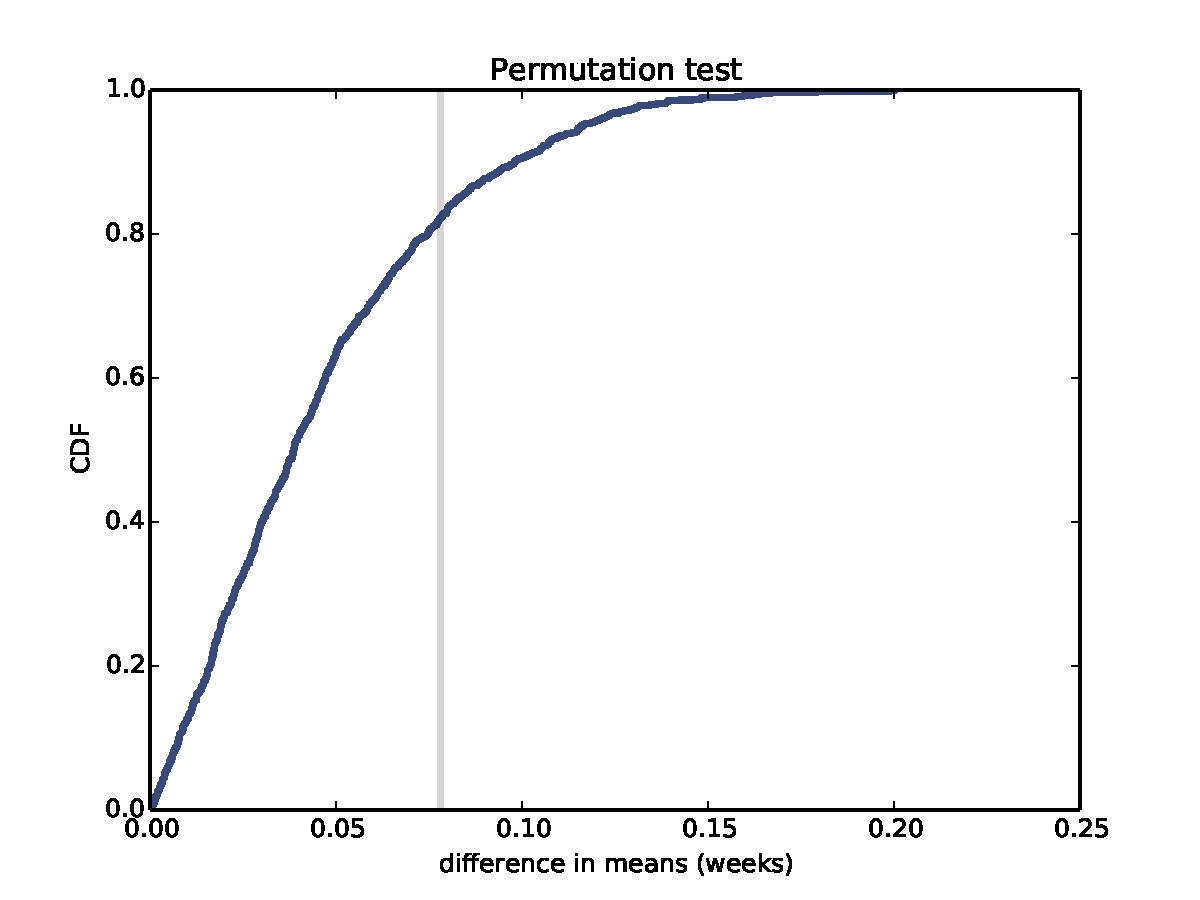
\includegraphics[height=2.5in]{figs/hypothesis1.pdf}}
\caption{귀무가설 아래 평균임신기간 차이 CDF.}
\label{hypothesis1}
\end{figure}

{\tt HypothesisTest}에는 {\tt PlotCdf}가 있는데 관측 효과 크기를 나타내는 회색선과 검정 통계량 분포를 플롯으로 그린다.
\index{thinkplot}
\index{HypothesisTest}
\index{Cdf}
\index{효과 크기 (effect size)}

\begin{verbatim}
    ht.PlotCdf()
    thinkplot.Show(xlabel='test statistic',
                   ylabel='CDF')
\end{verbatim}

그림~\ref{hypothesis1}에 결과가 있다.
CDF는 0.83에서 관측 차이와 교차하는데, p-값의 보수 0.17이다.

 shows the result.  The CDF intersects the
observed difference at 0.83, which is the complement of the p-value,
0.17.
\index{p-값 (p-value)}

만약 출생 체중으로 동일한 분석을 실행한다면, 계산된 p-값은 0 이다; 1000 번 시험 후에, 모의시험은 결코 관측 차이가 0.12 lbs 보다 큰 효과를 산출하지 못한다.
그래서, $p < 0.001$ 가 나오고, 출생 체중에 차이는 통계적으로 유의하다고 결론낸다. 

\index{출생 체중 (birth weight)}
\index{체중 (weight)!출생 (birth)}
\index{유의성 (significant)} 
\index{통계적 유의성 (statistically significant)}


\section{다른 검정 통계량 (ther test statistics)}

최선의 검정 통계량을 고르는 것은 무슨 질문을 하느냐에 달려 있다.
예를 들어, 만약 관련된 질문이 첫번째 아이에 대해서 임신 기간이 다른지에 관한 것이라면, 앞절에서 수행했던 것과 같이, 평균에 대해 차이 절대값을 검정하는 것이 의미가 있다.

\index{검정 통계량 (test statistic)}
\index{임신 기간 (pregnancy length)}

만약 첫번째 아이가 늦게 출생하는 경향이 있다고 생각할 이유가 있다면, 차이값의 절대값을 취하지 않는다; 대신에 다음 검정 통계량을 사용한다.

\begin{verbatim}
class DiffMeansOneSided(DiffMeansPermute):

    def TestStatistic(self, data):
        group1, group2 = data
        test_stat = group1.mean() - group2.mean()
        return test_stat
\end{verbatim}

{\tt DiffMeansOneSided}은 {\tt DiffMeansPermute}에서 {\tt MakeModel}와 {\tt RunModel}을 상속받는다; 유일한 차이는 {\tt TestStatistic}가 
차이에 절대값을 취하지 않는다는 것이다.
이런 유형의 검증을 {\bf 단측 (one-sided)} 검증이라고 한다. 왜냐하면,
차이 분포의 단측면만 고려하기 때문이다. 앞선 검정은 양쪽을 사용하기 때문에 {\bf 양측 (two-sided)} 검증이라고 한다.
\index{단측 검증 (one-sided test)}
\index{양측 검증 (two-sided test)}

이 버젼 검정에 대해서, p-값은 0.09 다. 일반적으로 단측 검정에 대한 p-값은 양측 검정에 대한 p-값의 약 절반이다. 물론 분포 모양에 달려있다.

\index{p-값 (p-value)}

단측 가설, 첫째 아이가 늦게 태어난다는 것이 양측 가설보다 좀더 구체적이다. 그래서 p-값이 더 작다. 하지만, 더 강한 가정에 조차도, 차이는 통계적으로 유의적이지 않다.

\index{유의성 (significant)} 
\index{통계적 유의성 (statistically significant)}

동일한 프레임워크(framework)를 사용해서 표준 편차에 차이도 검정할 수 있다. 
~\ref{visualization} 절에서 첫번째 아이가 늦게 혹은 빨리 출산할 것같은 증거를 일부 보았다. 그래서, 표준 편차가 좀더 클 것이라는 가설을 세울 수 있다. 다음에 이 가설을 시험하는 방법이 있다.

\index{표준 편차 (standard deviation)}

\begin{verbatim}
class DiffStdPermute(DiffMeansPermute):

    def TestStatistic(self, data):
        group1, group2 = data
        test_stat = group1.std() - group2.std()
        return test_stat
\end{verbatim}

이것은 단측 검정인데 이유는 가설이 첫번째 아이 집단에 대한 표준편차가 단지 다르다는 것이 아니라 더 높다는 것이다. p-값이 0.09로, 통계적으로 유의적이지 않다.

\index{p-값 (p-value)}
\index{순열 (permutation)}
\index{유의성 (significant)} 
\index{통계적 유의성 (statistically significant)}


\section{상관 검정 (Testing a correlation)}
\label{corrtest}

상기 프레임워크를 사용해서 상관도 검정할 수 있다. 
예를 들어, NSFG 데이터셋에서, 산모 나이와 출생 체중 사이 상관관계는 약 0.07 이다. 
나이가 많은 산모 아이가 더 체중이 나가는 것처럼 보인다. 하지만 이 효과가 우연에 의한 것일까요?
\index{상관 (correlation)}
\index{검정 통계량 (test statistic)}

검정 통계량으로, 피어슨 상관을 사용했지만, 스피어만 상관도 동일하게 동작한다. 만약 양의 상관 관계로 예측하는 합리적 논거가 있다면, 단측 검정을 할 수도 있다. 하지만, 그런 이유가 없기 때문에, 상관 절대값을 사용해서 양측검정을 수행한다.
\index{피어슨 상관계수 (Pearson coefficient of correlation)}
\index{스피어만 상관계수 (Spearman coefficient of correlation)}

귀무 가설은 산모 연령과 출생 체중 사이에 상관 관계가 없다는 것이다.
관측값을 뒤섞어서, 산모 연령과 출생 체중 분포가 같지만 변수 사이에 관련이 없는 세상을 모의 시험할 수 있다.
\index{출생 체중 (birth weight)}
\index{체중 (weight)!출생 (birth)}
\index{귀무 가설 (null hypothesis)}

\begin{verbatim}
class CorrelationPermute(thinkstats2.HypothesisTest):

    def TestStatistic(self, data):
        xs, ys = data
        test_stat = abs(thinkstats2.Corr(xs, ys))
        return test_stat

    def RunModel(self):
        xs, ys = self.data
        xs = np.random.permutation(xs)
        return xs, ys
\end{verbatim}

{\tt data}는 한쌍 시퀀스다. {\tt TestStatistic}가 피어슨 상관 절대값을 계산한다. {\tt RunModel}이 {\tt xs}를 뒤섞고 모의시험한 데이터를 반환한다.
\index{HypothesisTest}
\index{순열 (permutation)}
\index{피어슨 상관계수 (Pearson coefficient of correlation)}

다음에 데이터를 읽어 들이고, 시험을 수행하는 코드가 있다.

\begin{verbatim}
    live, firsts, others = first.MakeFrames()
    live = live.dropna(subset=['agepreg', 'totalwgt_lb'])
    data = live.agepreg.values, live.totalwgt_lb.values
    ht = CorrelationPermute(data)
    pvalue = ht.PValue()
\end{verbatim}

{\tt subset} 인자로 {\tt dropna}를 사용해서 필요한 변수 둘 중에서 결측된 행을 뺀다.
\index{dropna}
\index{NaN}
\index{결측값 (missing values)}

실제 상관계수는 0.07이다. 계산된 p-값은 0 이다; 1000 번 반복한 뒤에, 가장 큰 모의 시험 상관계수 p-값은 0.04다. 그래서, 관측된 상관계수가 작을지라도, 통계적 유의성이 있다.
\index{p-값 (p-value)}
\index{유의성 (significant)} 
\index{통계적 유의성 (statistically significant)}

``통계적 유의성 (statistically significant)''이 항상 효과가 중요하거나, 실무에서 유의적이라는 의미는 아니라는 것을 상기 예제가 상기 시킨다.
단지 유연으로 발생할 것 같지 않는다는 의미다.

\section{비율 검정 (Testing proportions)}
\label{casino}
\index{카이제곱 검정 chi-squared test}

카지노를 운영한다고 가정합시다. 그런데 고객 한명이 비뚤어진 주사위를 사용하고 있다고 용의선상에 올려놓는다; 즉, 다른 쪽보다 한쪽 면이 더 많이 나오도록 변형한 주사위. 주인장이 주장하는 사기꾼을 체포하고 주사위를 압수했다. 하지만, 이제 주사위가 비뚤어졌다는 것을 주인장이 증명해야 한다.
주사위를 60번 던져서 다음과 같은 결과를 얻었다.
\index{카지노 (casino)}
\index{주사위 (dice)}
\index{비뚤어진 주사위 (crooked die)}

\begin{center}
\begin{tabular}{|l|c|c|c|c|c|c|}
\hline
Value     &  1  &  2  &  3  &  4  &  5  &  6  \\ 
\hline
Frequency &  8  &  9  &  19  &  5  &  8  &  11  \\
\hline
\end{tabular}
\end{center}

평균적으로 주사위 각 값은 10번씩 나올 것으로 예상된다.
데이터셋에서, 값 3이 기대한 것보다 더 자주 나오고, 값 4는 덜 나오는 것 처럼 보인다.하지만, 이 차이가 통계적으로 유의적일까요?
\index{빈도 (frequency)}
\index{유의성 (significant)} 
\index{통계적 유의성 (statistically significant)}

가설을 검정하기 위해서, 각 값에 대한 기대 빈도, 기대 빈도와 관측 빈도 차이, 전체 절대값 차이를 계산할 수 있다. 상기 예제에서, 주사위 각 면은 60 회 중에서 10 회 나올 것으로 예상된다; 이 기대값에서 편차가 -2, -1, 9, -5, -2, 1 이 된다; 그래서 전체 절대값 차이는 20 이 된다. 우연히 이러한 차이를 얼마나 자주 목도할까?
\index{편차 (deviation)}

다음에 상기 질문에 대답하는 {\tt HypothesisTest} 버젼이 있다.
\index{HypothesisTest}

\begin{verbatim}
class DiceTest(thinkstats2.HypothesisTest):

    def TestStatistic(self, data):
        observed = data
        n = sum(observed)
        expected = np.ones(6) * n / 6
        test_stat = sum(abs(observed - expected))
        return test_stat

    def RunModel(self):
        n = sum(self.data)
        values = [1, 2, 3, 4, 5, 6]
        rolls = np.random.choice(values, n, replace=True)
        hist = thinkstats2.Hist(rolls)
        freqs = hist.Freqs(values)
        return freqs
\end{verbatim}

데이터는 빈도 리스트로 표현된다: 관측값은 {\tt [8, 9, 19, 5, 8, 11]}이 되고 ; 기대 빈도는 모두 10 이다.
검정 통계량은 절대값 차이의 총합이다.
\index{빈도 (frequency)}

귀무 가설은 주사위가 공정하다는 것으로 {\tt values} 에서 난수 표본을 뽑아 모의 시험한다. {\tt RunModel} 은 {\tt Hist}를 사용해서 계산하고, 빈도 리스트를 반환한다.

\index{Hist}
\index{귀무 가설 (null hypothesis)}
\index{모형 (model)}

이 데이터에 대한 p-값은 0.13으로 의미하는 바는 만약 주사위가 공정하다면, 전체 관측 편차를 약 13\% 가능성으로 볼 것으로 기대된다. 그래서, 명백한 효과는 통계적으로 유의하지 않다.
\index{p-값 (p-value)}
\index{편차 (deviation)}
\index{유의성 (significant)} 
\index{통계적 유의성 (statistically significant)}


\section{카이제곱 검정 (Chi-squared tests)}
\label{casino2}

이전 절에서 검정 통계량으로 총편차를 사용했다. 하지만,
비율을 검정하는데, 카이제곱 통계량을 사용하는 것이 좀더 일반적이다.
%
\[ \goodchi^2 = \sum_i \frac{(O_i - E_i)^2}{E_i} \]
%
%% TODO: Consider using upper case chi, which is more strictly correct,
%% but harder to distinguish from X.
% 

여기서, $O_i$는 관측빈도, $E_i$는 기대빈도다. 다음에 파이썬 코드가 있다.
\index{카이제곱 검정 (chi-squared test)}
\index{카이제곱 통계량 (chi-squared statistic)}
\index{검정 통계량 (test statistic)}

\begin{verbatim}
class DiceChiTest(DiceTest):

    def TestStatistic(self, data):
        observed = data
        n = sum(observed)
        expected = np.ones(6) * n / 6
        test_stat = sum((observed - expected)**2 / expected)
        return test_stat
\end{verbatim}

(절대값을 취하기 보다)편차를 제곱하면 큰 편차에 더 많은 가중치를 준다.
{\tt expected}로 나누게 되면 편차를 표준화한다. 이 경우에 기대 빈도가 모두 같아서 효과가 없다.

\index{편차 (deviation)}

카이제곱 통계량을 사용한 p-값은 0.04로 총편차를 사용해서 얻은 0.13보다도 훨씬 작다. 만약 5\% 분계점을 심각하게 생각한다면, 효과가 통계적으로 유의하다고 고려할 수 있다. 하지만, 검정 두가지를 모두 고려해서, 결과는 경계선에 있다고 말할 수 있다. 주사위가 삐뚤어졌다는 가능성을 배제하지는 않지만, 고발된 사기꾼에게 유죄 판결을 하지는 않을 것이다.

\index{p-값 (p-value)}
\index{유의성 (significant)} 
\index{통계적 유의성 (statistically significant)}

상기 예제는 중요한 점을 시연해 준다: p-값이 검정 통계량과 귀무 가설 모형에 달려있다. 그리고 때때로, 이러한 선택에 따라 효과가 통계적으로 유의성을 갖거나 갖지 않거나 결정된다.
\index{귀무 가설 (null hypothesis)}
\index{모형 (model)}


\section{다시 첫째 아이}

이장 앞에서 첫번째 아이와 첫째가 아닌 아이들에 대한 임신 기간을 살펴봤고, 평균과 표준편차에 명백한 차이는 통계적으로 유의적이지 않다고 결론냈다. 하지만, ~\ref{visualization} 절에서 평균 기간 분포에서 명백한 차이를 몇가지 봤다. 특히, 35주에서 43주차 범위에서 그렇다. 이러한 차이가 통계적 유의성이 있는지 살펴보기 위해서, 카이제곱 통계량에 기반한 검정을 사용할 수 있다.
\index{표준 편차 (standard deviation)}
\index{통계적 유의성 (statistically significant)} 
\index{유의성 (significant)}
\index{임신 기간 (pregnancy length)}

다음 코드는 앞선 예제로부터 요소를 결합한다.

\index{HypothesisTest}

\begin{verbatim}
class PregLengthTest(thinkstats2.HypothesisTest):

    def MakeModel(self):
        firsts, others = self.data
        self.n = len(firsts)
        self.pool = np.hstack((firsts, others))

        pmf = thinkstats2.Pmf(self.pool)
        self.values = range(35, 44)
        self.expected_probs = np.array(pmf.Probs(self.values))

    def RunModel(self):
        np.random.shuffle(self.pool)
        data = self.pool[:self.n], self.pool[self.n:]
        return data
\end{verbatim}

데이터는 두개 임신 기간 리스트로 표현된다. 귀무가설은
표본 모두 동일한 분포에서 추출되었다는 것이다.
{\tt MakeModel}은 {\tt hstack}을 사용해서 두 표본을 합동(pooling)해서 분포를 모형화한다. 그리고 나서, {\tt RunModel}은 합동 표본을 뒤섞고 이것을 두 부분으로 쪼갬으로써 모의 실험 데이터를 생성한다.
\index{귀무 가설 (null hypothesis)}
\index{모형 (model)}
\index{hstack}
\index{임신 기간 (pregnancy length)}

{\tt MakeModel}은 또한 {\tt values}를 정의하는데, 사용할 주차 범위가 되고, 
\verb"expected_probs"는 합동 분포(pooled distribution)에서 각 값의 확률이다.

다음에 검정 통계량을 계산하는 코드가 있다.

\begin{verbatim}
# class PregLengthTest:

    def TestStatistic(self, data):
        firsts, others = data
        stat = self.ChiSquared(firsts) + self.ChiSquared(others)
        return stat

    def ChiSquared(self, lengths):
        hist = thinkstats2.Hist(lengths)
        observed = np.array(hist.Freqs(self.values))
        expected = self.expected_probs * len(lengths)
        stat = sum((observed - expected)**2 / expected)
        return stat
\end{verbatim}

{\tt TestStatistic}은 첫째 아이와 첫째 아이가 아닌 아이들에 대한 카이제곱 통계량을 계산하고 더한다.
\index{카이제곱 통계량 (chi-squared statistic)}

{\tt ChiSquared}는 임신 기간 시퀀을 받아, 히스토그램을 계산하고,
{\tt observed}를 계산하는데, 이는 {\tt self.values}에 상응하는 빈도 리스트다. 기대 빈도 리스트를 계산하기 위해서, 표본 크기에 미리 계산된 확률 \verb"expected_probs"을 곱한다. 그러면 카이제곱 통계량 {\tt stat}을 반환한다.

NSFG 데이터에 대해서, 전체 카이제곱 통계량은 102로 그 자체로 많은 것을 의미하지는 않는다. 하지만, 1000회 반복 후에, 귀무가설 아래에서 가장 큰 검정 통계량은 32다. 관측 카이제곱 통계량이 귀무가설 아래에서 가능할 것 같지 않다고 결론내린다. 그래서, 외관 효과는 통계적 유의성이 있다.

\index{귀무 가설 (null hypothesis)}
\index{통계적 유의성 (statistically significant)} 
\index{유의성 (significant)}

이번 예제는 카이제곱 검정 한계를 보여준다: 두 집단 사이에 차이가 있다는 것을 나타내지만, 차이가 무엇인지에 관한 구체적인 어떤 것도 말하지는 못한다.

\section{오류 (Errors)}
\index{오류 (error)}

전통적인 가설 검정에서 만약 p-값이 특정 분계점, 흔히 5\% 보다 아래라면, 통계적 유이성이 있다고 본다. 이러한 절차는 두가지 질문을 불러온다.
\index{p-값 (p-value)}
\index{분계점 (threshold)}
\index{통계적 유의성 (statistically significant)} 
\index{유의성 (significant)}

\begin{itemize}

\item 만약 효과가 실제로 우연으로 인한다면, 효과를 잘못해서 유의적으로 고려할 확률은 얼마나 될까? 이 확률이 {\bf 거짓 양성률 (false positive rate)}이다.
\index{거짓 양성 (false positive)}

\item 만약 효과가 진실이라면, 가설 검정이 실패할 가능성은 얼마나 될까?
이 확률이 {\bf 거짓 음성률 (false negative rate)}이다.
\index{거짓 음성 (false negative)}

\end{itemize}

거짓 양성률은 상대적으로 계산하기 쉽다: 만약 분계점이 5\% 이면, 거짓 양성률은 5\% 다. 다음에 이유가 있다.

\begin{itemize}

\item 만약 실제 효과가 없다면, 귀무 가설은 사실이다. 그래서 귀무 가설을 모의 시험함으로써, 검정 통계량 분포를 계산할 수 있다. 이 분포를 $\CDF_T$ 라고 부른다.
\index{귀무 가설 (null hypothesis)}
\index{CDF}

\item 실험을 매번 실행할 때마다, 검정 통계량 $t$ 를 얻는데, $CDF_T$에서 뽑아낸 것이다. 그리고 나서, p-값을 계산하는데, $CDF_T$에서 나온 난수 값이 {\tt t}를 초과하는 확률이다. 그래서 $1 - CDF_T(t)$이 된다.

\item 만약 $CDF_T(t)$가 95\%보다 크다면, p-값이 5\% 보다 작다; 즉, 만약 $t$가 95번째 백분위수를 초과하면 그렇다. 그리고, $CDF_T$에서 고른 값이 95번째 백분위수를 얼마나 자주 초과할까? 거의 5\% 다.

\end{itemize}

그래서, 5\% 분계점을 가진 가설 검정을 수행한다면, 거짓 양성이 20번 중 1번 예상된다. 

\section{검정력 (Power)}
\label{power}

거짓 음성률은 계산하기 더 어렵다. 왜냐하면, 실제 효과 크기에 의존하고 정상적으로는 실제 효과 크기를 모르기 때문이다. 한가지 선택옵션은 가상 효과크기(hypothetical effect size) 조건으로 거짓 음성률을 계산하는 것이다.
\index{효과 크기 (effect size)}

예를 들어, 만약 두 집단 사이에 관측 차이가 정확하다면, 관측 표본을 모집단 모형으로 사용해서 모의 시험 데이터로 가설 검정을 실행할 수 있다.
\index{모형 (model)}

\begin{verbatim}
def FalseNegRate(data, num_runs=100):
    group1, group2 = data
    count = 0

    for i in range(num_runs):
        sample1 = thinkstats2.Resample(group1)
        sample2 = thinkstats2.Resample(group2)

        ht = DiffMeansPermute((sample1, sample2))
        pvalue = ht.PValue(iters=101)
        if pvalue > 0.05:
            count += 1

    return count / num_runs
\end{verbatim}

{\tt FalseNegRate}는 각 집단마다 하나씩 두 시퀀스 형태로 데이터를 받는다.

루프를 매번 돌 때마다, 각 집단에서 난수 표본을 뽑아서 가설 검정을 실행함으로써 실험을 모의 시험한다. 그리고 나서 결과를 확인하고 거짓 음성 갯수를 계수한다.
\index{Resample}
\index{순열 (permutation)}

{\tt Resample}은 시퀀스를 받아 복원 추출로 동일 길이를 가진 표본을 뽑는다.
\index{복원 (replacement)}

\begin{verbatim}
def Resample(xs):
    return np.random.choice(xs, len(xs), replace=True)
\end{verbatim}

다음에 임신 기간을 검정하는 코드가 있다.

\begin{verbatim}
    live, firsts, others = first.MakeFrames()
    data = firsts.prglngth.values, others.prglngth.values
    neg_rate = FalseNegRate(data)
\end{verbatim}

결과가 약 70\%로 의미하는 바는 만약 평균 임신기간에 실제 차이가 0.078 주라면, 이 표본 크기를 가진 실험은 대략 70\% 음성 검정을 산출할 것으로 기대된다.
\index{임신 기간 (pregnancy length)}

이 결과는 종종 다르게 제시된다: 만약 실제 차이가 0.078 주라면, 
대략 30\% 만 양성 검정을 기대해야 한다. 
이 ``정확한 양성률 (correct positive rate)''이 검정 {\bf 검정력(power)}이라고 부르고, 종종 ``민감도 (sensitivity)''라고 한다. 주어진 크기 효과를 탐지하는 검정 능력을 반영한다.
\index{검정력 (power)}
\index{민감도 (sensitivity)}
\index{정확한 양성 (correct positive)}

이 예제에서, 검정은 단지 30\% 가능성만으로 양성 결과를 산출한다(다시, 차이가 0.078 주라는 것을 가정하면). 경험 법칙으로, 80\% 검정력이 납득할 수 있는 수준이다. 그래서 이 검정은 ``검정력 부족 (underpowered)''하다고 말할 수 있다.
\index{검정력 부족 (underpowered)}

일반적으로 음성 가설 검정이 두 집단 사이에 차이가 없다는 것을 의미하는 것은 아니다; 대신에 만약 차이가 있다면, 너무 작아서 표본크기로 탐지할 수 없다는 것을 제시한다.

\section{반복 (Replication)}
\label{replication}

이번 장에서 시연한 가설검정과정은 엄밀히 말하면 좋은 관례(good practice)는 아니다.

첫째, 다중 검정(multiple tests)을 수행했다. 만약 가설 검정 하나를 실행한다면, 거짓양성(false positive) 가능성은 약 20번 중에 한번으로 수용가능하다. 하지만, 20번 검정을 수행한다면, 대부분 적어도 한번은 거짓양성을 예상해야한다.
\index{다중 검정 (multiple tests)}

둘째, 탐색과 검정에 동일한 데이터셋을 사용했다. 만약 대용량 데이터셋을 탐색하고, 놀라운 효과를 발견하고 나서, 효과가 유의성이 있는지 검정한다면, 거짓 양성(false positive)을 생성할 가능성이 있다.

\index{통계적 유의성 (statistically significant)} 
\index{유의성 (significant)}

다중 검정을 보상하기 위해서, p-값 분계점을 조정할 수 있다. (\url{https://en.wikipedia.org/wiki/Holm-Bonferroni_method} 참조). 혹은, 한 데이터셋은 탐색, 다른 데이터셋은 검정으로 데이터를 분할해서 두 문제를 다룰 수 있다. 
\index{p-값 (p-value)}
\index{홈-본페로니 법 (Holm-Bonferroni method)}

몇몇 분야에서는 이러한 관례가 요구되고 있거나 적어도 장려한다. 하지만, 이러한 문제를 암묵적으로 출판된 결과를 반복(replication)하면서 다루는 것도 흔하다. 전형적으로, 새로운 결과를 보고하는 첫번째 논문은 탐색적으로 고려된다. 새로운 데이터로 결과를 반복하는 이어지는 논문은 확증적(confirmatory)으로 고려된다.
\index{확증적 결과 (confirmatory result)}

공교롭게도, 이 장에서 결과를 반복할 기회가 있다.
이책 첫번째 판은 2002년에 나온 NSFG 사이클 6에 기반했다.
2011년 10월 CDC가 2006--2010에 실시한 인터뷰에 기반한 추가 데이터를 출시했다. {\tt nsfg2.py} 에는 이 데이터를 읽고 정제한 코드가 포함되어 있다. 새로운 데이터셋으로 분석한 결과는 다음과 같다.
\index{NSFG}

\begin{itemize}

\item 평균 임신 기간에 차이는 0.16 주다. $p < 0.001$ 으로 통계적 유의성이 있다. (원본 데이터셋 0.078주와 비교된다.)

\index{통계적 유의성 (statistically significant)} 
\index{유의성 (significant)}
\index{임신 기간 (pregnancy length)}

\item 출생 체중에 차이는 0.17 파운드로 $p < 0.001$ 이다.
(원본 데이터셋 0.12 lbs와 비교된다.)
\index{출생 체중 (birth weight)}
\index{체중 (weight)!출생 (birth)}

\item 출생 체중과 산모 연령 사이 상관계수는 0.08 로 $p < 0.001$ 이다. (0.07과 비교된다.).

\item 카이제곱검정은 $p < 0.001$ 으로 통계적 유의성이 있다.
$p < 0.001$ (원본 데이터도 그렇다.).

\end{itemize}

요약하면, 원본 데이터에서 통계적 유의성이 있는 모든 효과가 새로운 데이터셋에서도 반복되었다. 그리고 임신기간에 차이는 원데이터에서 유의성이 없었으나 새로운 데이터셋에서는 더 커졌고 유의성이 있다.


\section{연습 문제}

이 연습문제에 대한 해답은 \verb"chap09soln.py" 파일에 나와있다.

\begin{exercise}
표본크기가 증가함에 따라, 가설검정력은 증가하는데,
효과가 실제하면 좀더 양성임을 의미한다.
반대로, 표본크기가 줄어들면, 검정력은 설사 효과가 실제한다고 하더라도 덜 양성일 것 같다.
\index{표본크기}

이런 작동방식을 조사하는데, NSFG 데이터에서 다른 일부 데이터를 갖는 검정을 실시한다.
{\tt thinkstats2.SampleRows}을 사용해서, 데이터프레임에 임의로 행일부를 선택한다.

\index{가족성장 국가조사}
\index{NSFG}
\index{데이터프레임}

표본크기가 감소함에 따라 검정 p-값에는 무슨 일이 일어나는가?
양의 검정을 산출하는 최소 표본크기는 얼마인가?

\index{p-값}
\end{exercise}


\begin{exercise}

\ref{testdiff}~절에서, 
순열로 귀무가설을 모의시험했다; 즉,
관측된 값을 마치 전체 모집단을 대표하는 것처럼 다루었고,
무작위로 모집단의 구성원을 두 집단에 배정했다.
\index{귀무가설}
\index{순열}

대안은 표본을 사용해서 모집단 분포를 추정하고 나서, 분포로부터 임의 표본을 추출하는 것이다.
이런 과정을 {\bf 재표집(resampling)}이라고 부른다.
재표집을 구현하는 몇가지 방식이 있지만, 가장 단순한 것중 하나가 \ref{power}~처럼 관측된 값에서 복원방식으로 표본을 추출하는 것이다.

\index{재표집}
\index{복원}

{\tt DiffMeansPermute}에서 상속받고, 순열보다 재표집을 구현하는 {\tt RunModel}을 
치환(override)하는 클래스 {\tt DiffMeansResample}을 작성하시오.
\index{순열}

이 모형을 사용해서 임신기간과 출생체중 사이 차이를 검정하시오.
이 모형이 결과에 얼마나 영향을 주는가?
\index{모형}
\index{출생체중}
\index{체중!출생}
\index{임신기간}

\end{exercise}


\section{용어 사전}

\begin{itemize}

\item 가설 검정 (hypothesis testing): 외관 효과(apparent effect)가 통계적 유의성이 있는지 결정하는 과정.
\index{가설 검정 (hypothesis testing)}

\item 검정 통계량 (test statistic): 효과 크기를 정량화하는데 사용되는 통계량.
\index{검정 통계량 (test statistic)}
\index{효과 크기 (effect size)}

\item 귀무 가설 (null hypothesis): 외관 효과가 우연에 의한 것이라는 가정에 기반한 시스템 모델.
\index{귀무 가설 (null hypothesis)}

\item p-값 (p-value): 효과가 우연에 의해서 발생한 확률.
\index{p-값 (p-value)}

\item 통계적 유의성 (statistically significant): 우연에 의해서 발생할 것 같지 않다면, 효과는 통계적 유의성이 있다.
\index{통계적 유의성 (statistically significant)} 
\index{유의성 (significant)}

\item 순열 검정 (permutation test): 관측 데이터셋에서 순열을 생성해서 p-값을 계산하는 방법.
\index{순열 검정 (permutation test)}

\item 재표본 검정 (resampling test): 관측 데이터셋에서 복원으로 표본을 생성해서 p-값을 계산하는 방법.
\index{재표본 검정 (resampling test)}

\item 양측 검정 (two-sided test): ``효과 크기가 양으로 혹은 음으로 관측 효과보다 얼마나 큰가?'' 를 묻는 검정.

\item 단측 검정 (one-sided test): ``효과 크기가 동일 부호로 관측 효과보다 얼마나 큰가?'' 를 묻는 검정.
\index{단측 검정 (one-sided test)}
\index{양측 검정 (two-sided test)}
\index{검정 (test)!단측 (one-sided)}
\index{검정 (test)!양측 (two-sided)}

\item 카이-제곱 검정 (chi-squared test): 검정 통계량으로 카이-제곱 통계량을 사용하는 검정.
\index{카이-제곱 검정 (chi-squared test)}

\item 거짓 양성 (false positive): 사실이 아닐 때, 효과가 사실이라는 결론.
\index{거짓 양성 (false positive)}

\item 거짓 음성 (false negative): 우연이 아닐 때 효과가 우연 때문이라는 결론.
\index{거짓 음성 (false negative)}

\item 검정력 (power): 대립가설이 사실일 때, 이를 사실로서 결정할 확률이다. 검정력이 90\%라고 하면, 대립가설이 사실임에도 불구하고 귀무가설을 채택할 확률은 10\%이다.\footnote{\url{http://ko.wikipedia.org/wiki/검정력} 참조}
\index{검정력 (power)}
\index{귀무 가설 (null hypothesis)}

\end{itemize}



